\sectionframe{Original Model}

\section{Original Model}

\begin{frame}{Original Model Problem Domain}
	Power Converter AC $\to$ DC.
	Types:
	\begin{itemize}
		\item fixed frequency
		\item variable frequency ($\leftarrow$ the model describes this type)
	\end{itemize}

	\vspace{2em}
	Model maps
	\begin{itemize}
		\item Input: Point at which the converter switched the last time $\theta \in [0, 2 \pi)$
		\item Ouput: Point at which the converter will switch the next time $F(\theta) \in [0, 2 \pi)$
	\end{itemize}
\end{frame}

\begin{frame}{Original Model Definition (1/3)}
	\vspace{-3.0em}
	\begin{align}
		\theta \mapsto F(\theta)
	\end{align}
	\begin{align}
		F(\theta) = \begin{cases}
			            F_1(\theta) & \text{if } q \cdot \cos(\theta) > 0 \\
			            F_2(\theta) & \text{if } q \cdot \cos(\theta) < 0
		            \end{cases}
	\end{align}
	\begin{align}
		F_1(\theta) & = \begin{cases}
			                \theta + z_{L_+} + z_1 & \text{if } z_{L_+} < z_{L_0} \\
			                \theta + z_{L_0} + z_2 & \text{if } z_{L_+} > z_{L_0}
		                \end{cases}
	\end{align}
	\begin{align}
		F_1(\theta) & = \begin{cases}
			                \theta + z_{R_+} + z_3 & \text{if } z_{R_+} < z_{R_0} \\
			                \theta + z_{R_0} + z_4 & \text{if } z_{R_+} > z_{R_0}
		                \end{cases}
	\end{align}
\end{frame}

\begin{frame}{Original Model Definition (2/3)}
	\vspace{-3.0em}
	\begin{subequations}
		\begin{align}
			(q \cdot \cos(\theta) + \mu \cdot \chi) \cdot e^{\lambda \cdot z_{L_+}}
			 & = q \cdot \cos(\theta + z_{L_+} + z_1) + \mu \cdot \chi \\
			(q \cdot \cos(\theta) + \mu \cdot \chi) \cdot e^{\lambda \cdot z_{L_0}}
			 & = q \cdot \cos(\theta + z_{L_0} + z_1) - \mu \cdot \chi \\
			(q \cdot \cos(\theta) + \mu \cdot \chi) \cdot e^{\lambda \cdot z_{R_+}}
			 & = q \cdot \cos(\theta + z_{R_+} + z_1) + \mu \cdot \chi \\
			(q \cdot \cos(\theta) + \mu \cdot \chi) \cdot e^{\lambda \cdot z_{R_0}}
			 & = q \cdot \cos(\theta + z_{R_0} + z_1) - \mu \cdot \chi
		\end{align}
	\end{subequations}
	\begin{subequations}
		\begin{align}
			(q \cdot \cos(\theta + z_{L_+}) + \chi + 1) \cdot e^{\lambda \cdot z_1} - 1
			 & = q \cdot  \cos(\theta + z_{L_+} + z_1) + \mu \cdot \chi \\
			(q \cdot \cos(\theta + z_{L_0}) + \chi + 1) \cdot e^{\lambda \cdot z_2} + 1
			 & = q \cdot  \cos(\theta + z_{L_0} + z_2) - \mu \cdot \chi \\
			(q \cdot \cos(\theta + z_{R_+}) + \chi + 1) \cdot e^{\lambda \cdot z_3} - 1
			 & = q \cdot  \cos(\theta + z_{L_+} + z_3) + \mu \cdot \chi \\
			(q \cdot \cos(\theta + z_{R_0}) + \chi + 1) \cdot e^{\lambda \cdot z_4} + 1
			 & = q \cdot  \cos(\theta + z_{R_0} + z_4) - \mu \cdot \chi
		\end{align}
	\end{subequations}
\end{frame}

\begin{frame}{Original Model Definition (3/3)}
	\vspace{-3.0em}
	\begin{align}
		\chi    & = \dfrac{R \cdot \chi_0}{\beta \cdot E_0} \\
		\lambda & = \dfrac{-R}{L \cdot 2 \cdot \pi \cdot f} \\
		q       & = \dfrac{R \cdot V_m}{\beta \cdot E_0}
	\end{align}

	Parameters varied in the 2D scan above:
	\begin{align*}
		E_0, \chi_0
	\end{align*}

	Symmetry in this model:
	\begin{align}
		F(\theta + \pi) = F(\theta) + \pi \mod 2 \pi
	\end{align}
\end{frame}

\begin{frame}{Original Model}
	\vspace{-2.0em}
	\begin{figure}
		\centering
		\subfloat[Full Model]{
			\includegraphics[height=0.6 \textheight]{99_Yunus/2D_Period_Zoomed/result.png}
		}
		\subfloat[Halved Model]{
			\includegraphics[height=0.6 \textheight]{98_Yunus_modpi/2D_Period_Zoomed/result.png}

		}
		\caption{2D Scan of Original Model}
	\end{figure}
\end{frame}

\begin{frame}{Original Model}
	\vspace{-3.0em}
	\begin{figure}
		\centering
		\subfloat[At Point $A$]{
			\includegraphics[width=0.6 \textheight]{99_Yunus/Period12/Cobweb_A_12/result.png}
		}
		\subfloat[At Point $B$]{
			\includegraphics[width=0.6 \textheight]{99_Yunus/Period12/Cobweb_B_12/result.png}
		}
		\subfloat[At Point $D$]{
			\includegraphics[width=0.6 \textheight]{99_Yunus/Period12/Cobweb_C_12/result.png}
		}
		\caption{Cobwebs of Original Model}
	\end{figure}
\end{frame}

\begin{frame}{Parameter Regions in Original Model}
	\begin{itemize}
		\item ``Type A'': At points $A$ and $B$ in 2D scan
		      \begin{itemize}
			      \item One cycle
			      \item Symmetrical
			      \item Example at point $A$: $\Cycle{\A^3\B^3\C^3\D^3}$
			      \item Example at point $C$: $\Cycle{\A^2\B^4\C^2\D^4}$ \vspace*{1em}
		      \end{itemize}
		\item ``Type B'': At point $B$ in 2D scan
		      \begin{itemize}
			      \item Two coexisting cycles
			      \item Asymmetrical
			      \item Example at point $B$: $\Cycle{\A^3\B^3\C^2\D^4}$ and $\Cycle{\A^2\B^4\C^3\D^3}$
		      \end{itemize}
	\end{itemize}
\end{frame}

\begin{frame}{Original Model Effects of Parameters}
	\vspace{-3.0em}
	\begin{figure}
		\centering
		\subfloat[Directions]{
			\includegraphics[width=0.6 \textheight]{99_Yunus/2D_Period_Zoomed_EffectsSingle/result.png}
		}
		\subfloat[Evolution for Parameter $E_0$]{
			\includegraphics[width=0.6 \textheight]{99_Yunus/ParameterEffects/E0/illustration.png}
		}
		\subfloat[Evolution for Parameter $\chi_0$]{
			\includegraphics[width=0.6 \textheight]{99_Yunus/ParameterEffects/hi/illustration.png}
		}
		\caption{Effects of the Individual Parameters on the Function of the Original Model}
	\end{figure}
\end{frame}
